\documentclass[conference]{IEEEtran}
\IEEEoverridecommandlockouts
%Template version as of 6/27/2024

\usepackage{cite}
\usepackage{amsmath,amssymb,amsfonts}
\usepackage{algorithmic}
\usepackage{graphicx}
\usepackage{textcomp}
\usepackage{xcolor}
\usepackage{tikz}
\usepackage{orcidlink}
\hypersetup{
    colorlinks=false,
    pdfborder={0 0 0},
}

\newcommand{\TODO}[1]{\textbf{\textcolor{red}{TODO: #1}}}

\def\BibTeX{{\rm B\kern-.05em{\sc i\kern-.025em b}\kern-.08em
    T\kern-.1667em\lower.7ex\hbox{E}\kern-.125emX}}

\begin{document}

\title{
    Investigating Protein Folding Dynamics Using Molecular Dynamics Simulations-based Approaches
}

\author{\IEEEauthorblockN{Christian Nix\,\orcidlink{0009-0006-5718-3452}}
\IEEEauthorblockA{\textit{School of Computation, Information and Technology (CIT)} \\
\textit{Technical University of Munich}\\
Munich, Germany \\
christian.nix@tum.de}
}

\maketitle

\begin{abstract}
\TODO{Lorem ipsum dolor sit amet, consetetur sadipscing elitr, sed diam nonumy eirmod tempor invidunt ut labore et dolore magna aliquyam erat, sed diam voluptua. At vero eos et accusam et justo duo dolores et ea rebum. Stet clita kasd gubergren, no sea takimata sanctus est Lorem ipsum dolor sit amet. Lorem ipsum dolor sit amet, consetetur sadipscing elitr, sed diam nonumy eirmod tempor invidunt ut labore et dolore magna aliquyam erat, sed diam voluptua. At vero eos et accusam et justo duo dolores et ea rebum. Stet clita kasd gubergren, no sea takimata sanctus est Lorem ipsum dolor sit amet. Lorem ipsum dolor sit amet, consetetur sadipscing elitr, sed diam nonumy eirmod tempor invidunt ut labore et dolore magna aliquyam erat, sed diam voluptua. At vero eos et accusam et justo duo dolores et ea rebum. Stet clita kasd gubergren, no sea takimata sanctus est Lorem ipsum dolor sit amet. Duis autem vel eum iriure dolor in hendrerit in vulputate velit esse molestie consequat, vel illum dolore eu feugiat nulla facilisis at vero eros et accumsan et iusto odio dignissim qui blandit praesent luptatum zzril delenit augue duis dolore te feugait nulla facilisi.}
\end{abstract}

\begin{IEEEkeywords}
\TODO{Index words to be added in the end.}
\end{IEEEkeywords}

\section{Introduction}
Proteins are fundamental in driving biological processes and form the basic building blocks that life relies on \cite{eisenberg2000protein}. They are pivotal in almost all cellular processes, thus motivating their study in fields such as medicine, chemistry, or biophysics. Proteins play essential roles in regulation, transportation, signaling, immune responses, and metabolism, among others. \cite[pp.~163ff., pp.~225ff.]{buxbaum2007fundamentals} Chemically, proteins are a polymer of 20 canonical amino acids that have unique side-chains giving them unique chemical properties, such as hydrophobicity, charge, or polarity. Neighboring amino acids are linked via peptide bonds formed between their \textit{amino} and carboxyl (\textit{acid}) groups, thus forming the protein's backbone from which their distinct side-chains extend. \cite{stollar2020uncovering}

Protein structure is commonly described as four hierarchical levels: primary, secondary, tertiary, and quaternary structure. The \textit{primary structure} refers to the linear sequence of amino acids in the protein chain. Given the chemical properties of neighboring amino acids, \textit{secondary structure} elements, such as $\alpha$-helices or $\beta$-sheets, can be formed. The secondary structure is stabilized by hydrogen bonds between backbone atoms. The \textit{tertiary structure} describes the overall 3D arrangement of the protein chain, including the side-chains, i.e., the determination of all atoms in 3D space. The tertiary structure is stabilized by a broad set of interactions, such as van der Waals forces, hydrogen bonds, ionic interactions, and disulfide bridges. Finally, some proteins consist of multiple polypeptide chains (i.e., multiple protein subunits), whose arrangement is described by the \textit{quaternary structure}. \cite[pp.~65ff.]{kessel2018introduction}

Generally speaking, protein function, and thus the protein's biochemical role, is determined by its 3D structure, motivating the study of protein structures and how proteins assume these structures \cite{lee2007predicting}. However, proteins are not static entities, but rather dynamic molecules that can undergo conformational changes to perform their functions. Therefore, understanding protein dynamics is crucial for a comprehensive understanding of protein function. \cite{teilum2009functional} Additionally, misfolded proteins can lead to various diseases, such as Alzheimer's, Parkinson's, or cystic fibrosis, further highlighting the importance of understanding protein folding as a dynamic process \cite{valastyan2014mechanisms}.

\subsection{Protein Folding and its Importance}
So far, we have established that knowing the 3D structure of proteins is important for understanding their function and role in biological processes. However, the process of protein folding itself is highly complex and not yet fully understood \cite{tsuboyama2023mega}. Anfinsen's Nobel prize-winning work demonstrated that the primary structure (i.e., the amino acid sequence) of a protein determines its final 3D structure, implying that all information necessary for folding is self-contained \cite{anfinsen1973principles}. However, if a protein were to randomly sample all possible conformations its primary sequence could take, the time required to fold would be much beyond the biologically relevant timescales (milliseconds to seconds) observed in nature \cite{levinthal1969fold, dobson2003protein}. For example, assuming 10 possible configurations per amino acid residue, a small protein of 100 residues would have $10^{100}$ possible conformations. A rotation around a single bond takes roughly $10^{-12}$ s \cite{lee2025ultrafast}, leading to a total time of $10^{88}$ s or roughly $10^{80}$ years to sample all conformations. This discrepancy is known as Levinthal's paradox \cite{levinthal1969fold}. Since we know that proteins do fold on biologically relevant timescales, there must be some guiding principles that direct the folding process efficiently.

To describe the folding process and its driving forces, we make use of the Gibbs free energy $G = H - TS$, where $H$ is the enthalpy, $T$ the temperature, and $S$ the entropy \cite[pp.~76ff.]{AtkinsDePaula2006}. The Gibbs energy is valid, because folding occurs at constant pressure and temperature \cite{ghelis2012protein, pain2000mechanisms, bryngelson1995funnels}. As becomes apparent from the definition of $G$, folding is driven by enthalpic ($H$) and entropic contributions ($TS$). For example, a main driver of folding is the hydrophobic effect, where non-polar residues cluster together \cite{durell2017hydrophobic}. This benefits the enthalpy via van der Waals forces between the residues, but also increases the entropy by releasing ordered water molecules into the bulk solvent \cite[pp.~280ff.]{KlostermeierRudolph2024}. If we now consider the free energy as a function of the protein's conformation, we arrive at the concept of the energy landscape of protein folding. In Levinthal's paradox, the energy landscape was assumed to be flat, with only the native, folded state being energetically favorable, resulting in random searching. During the 1990s, the concept of the energy landscape as a folding funnel was introduced (Figure \ref{fig:intro:funnel}). \cite{bryngelson1995funnels, onuchic1997theory}

\begin{figure}[b]
    \centering
    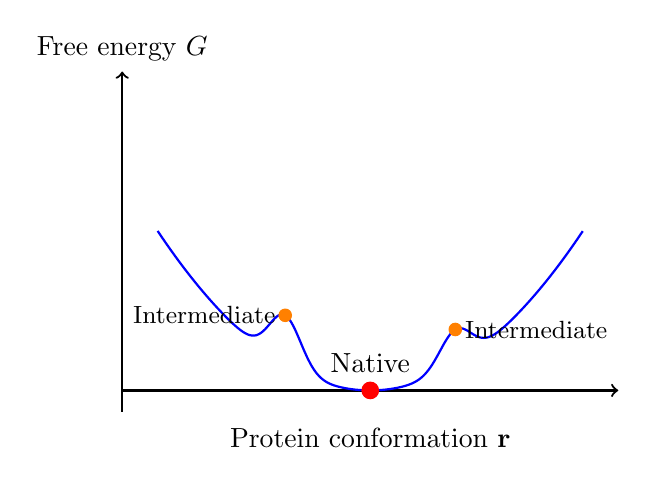
\begin{tikzpicture}[scale=1.5]
  % Define scaling factors
  \def\xscale{0.6}
  \def\yscale{0.6}
  
  % Function: f(x) = 0.25*x^2 + 0.7*exp(-10*(x+1.2)^2) + 0.5*exp(-10*(x-1.2)^2)
  % This creates a quadratic well with two local minima (intermediates)
  
  % Draw axes
  \draw[->, thick] (-3.5*\xscale,0) -- (3.5*\xscale,0) node[right] {};
  \draw[->, thick] (-3.5*\xscale,-0.3*\yscale) -- (-3.5*\xscale,4.5*\yscale) node[above] {Free energy $G$};
  
  % Plot the energy landscape
  \draw[thick, blue, smooth] plot[domain=-3:3, samples=100] 
    ({(\x)*\xscale}, {(0.25*\x*\x + 0.7*exp(-10*(\x+1.2)*(\x+1.2)) + 0.5*exp(-10*(\x-1.2)*(\x-1.2)))*\yscale});
  
  % Mark the native state (global minimum at x=0)
  \filldraw[red] (0,0) circle (2pt);
  \node[above=3pt] at (0,0) {Native};
  \node[below=10pt] at (0,0) {Protein conformation $\mathbf{r}$};
  
  % Mark intermediate states (local minima at x ≈ ±1.2)
  \filldraw[orange] ({-1.2*\xscale},{(0.25*1.44 + 0.7)*\yscale}) circle (1.5pt);
  \node[left, font=\small] at ({-1.2*\xscale},{(0.25*1.44 + 0.7)*\yscale}) {Intermediate};
  
  \filldraw[orange] ({1.2*\xscale},{(0.25*1.44 + 0.5)*\yscale}) circle (1.5pt);
  \node[right, font=\small] at ({1.2*\xscale},{(0.25*1.44 + 0.5)*\yscale}) {Intermediate};
  
\end{tikzpicture}
    \caption{\TODO{Temporary Fig} Schematic representation of a high-dimensional protein folding funnel which is a free energy function $G$ of protein conformation $\mathbf{r}$. The native state corresponds to the global minimum of the free energy. Local minima represent meta-stable folding intermediates which originate from conformational changes. Kinetic conversion between minima requires overcoming energy barriers and can thus be slow.}
    \label{fig:intro:funnel}
\end{figure}

As can be seen in Figure \ref{fig:intro:funnel}, the folding funnel concept correctly captures that conformations along a folding pathway do not have the same energy. The idealized funnel shape arises from the assumption that each newly formed native contact (i.e., a contact that exists in the native structure) lowers the free energy, leading to a monotonic decrease in free energy as folding progresses. \cite[pp.~283ff.]{KlostermeierRudolph2024} However, the energy landscape is much more rugged in reality, with many local extrema. For example, conformations stemming from rotating a side-chain may differ by small differences in energy, thus these conformations are interconverted rapidly. On the other hand, larger conformational changes, such as forming or breaking tertiary structure elements, may lead to greater energy changes and therefore result in local minima that are harder to escape from. \cite{bryngelson1995funnels} These local minima, given sufficiently large energy barriers, can lead to meta-stable states and folding intermediates \cite{dill2008protein}.

The protein folding problem is not limited to predicting the final folded structure, but is also interested in understanding the folding pathways, i.e., the process by which a protein transitions from its unfolded to folded state through these various intermediates and meta-stable states \cite{eaton2000fast}. Ground-breaking methods such as AlphaFold \cite{senior2020improvedAF1, jumper2021highlyAF2, abramson2024accurateAF3} have essentially solved the prediction of the final folded structure, although they do not reveal \emph{how} proteins reach that state \cite{outeiral2022current}. Importantly, proteins do not necessarily fold via a single, well-defined pathway, but can utilize multiple pathways to reach the native state \cite{sridevi2004increasing}. As a result, we must identify not only the final native state, but also the various folding intermediates along the pathways and determine the kinetics of folding, i.e., the rates at which transitions between conformational states occur, especially those that are rate-limiting and therefore control the overall folding speed \cite{gelman2014fast}.

\subsection{Studying Protein Folding Dynamics}
\label{sec:intro:studying_folding}
Until the 1990s, protein folding dynamics were primarily studied experimentally using \textit{stopped-flow} techniques, which allowed a temporal resolution of around 1 ms \cite{gibson19696}. At the same time, atomistic molecular dynamics (MD) simulations were limited to nanosecond timescales. As a result, all (at the time) described protein folding events occurred on timescales inaccessible to MD simulations. \cite{eaton2021modern} However, the development of laser-based temperature-jump (T-jump) techniques enabled the experimental study of protein folding on nanosecond timescales \cite{phillips1995ultrafast}. Nonetheless, T-jump experiments cannot provide information about the underlying conformational rearrangements as they report only global relaxation kinetics \cite{eaton2021modern}. In contrast, experimental methods such as Förster resonance energy transfer (FRET) can yield insights into the distances between specific residues, thus providing some structural information \cite{schuler2008protein}. However, experimental methods are generally limited in the level of detail they can provide about the folding process, motivating the use of MD simulations to allow atomistic insights into folding dynamics \cite{piana2014assessing}.

In molecular dynamics, the motion of atoms is propagated using classical mechanics, by integrating, e.g., Newton’s equations of motion \cite[pp.~358ff.]{santamaria2023molecular}. The forces acting on the atoms are typically obtained from a molecular mechanics force field\footnote{Since MD simulations are fully controlled by the user, the forces acting on the system do not have to correspond strictly to physical reality but can also be altered, e.g., by mixing classical mechanics with quantum mechanical effects \cite{warshel1976theoretical}.}, which provides an approximate potential energy function \cite[pp.~298ff.]{santamaria2023molecular}. As a result, running MD simulations allows us to explore the conformational space according to the Boltzmann distribution (given some assumptions, which we will discuss later), which includes folding events \cite{henin2022enhanced}. However, the exploration of conformational space is still stochastic, requiring us to run simulations for long enough. With increasing computational power \cite{salomon2013routine}, the use of specialized hardware \cite{shaw2008anton}, or highly parallelized simulations \cite{shirts2000screen}, MD simulations can access increasingly long timescales. \cite{hollingsworth2018molecular} Alternatively, enhanced sampling methods such as metadynamics \cite{laio2002escaping} or umbrella sampling \cite{torrie1977nonphysical} can be used to accelerate the exploration of rare conformations by biasing the sampling process, e.g., by adding biasing potential that guides the system over energy barriers \cite{henin2022enhanced}. However, since these methods bias the simulation, the downstream analysis of the resulting trajectories must be adapted accordingly \cite{kamenik2022enhanced}.

To extract meaningful insights from MD simulations, their trajectories must be analyzed appropriately. Some properties, such as the temperature, pressure, or distances, can be computed directly from (averages over) the frames of the trajectory. However, many properties of interest, such as free energies which determine folding pathways and their kinetics, depend not on the frames directly, but rather on the distribution of conformations they represent, i.e., the accessible conformational space. \cite[pp.~167ff.]{frenkel2002understanding} Analyzing the conformational space is non-trivial due to its high dimensionality (e.g., three spatial coordinates per atom). To enable interpretation, we can project the high-dimensional conformational space onto fewer collective variables (CVs), along which we, for example, can compute free energy surfaces (FES). \cite{fiorin2013using} Collective Variables are detailed in Section \TODO{Ref}. For extracting long-timescale kinetics, a probabilistic framework such as Markov State Models (MSMs) can be applied \cite{malmstrom2014application}. These will be discussed in detail in Section \TODO{Ref}. MSMs discretize the conformational space into distinct states, enabling the quantitative prediction of transition rates and folding pathways \cite{chodera2014markov}.

\subsection{Aim and Scope}
This work provides a literature review on computational approaches for investigating protein folding dynamics. We focus specifically on the transfer operator formalism which we summarize for the reader and afterwards leverage as a unifying link between different analysis techniques.

We examine two primary methods for extracting insight from molecular dynamics data. The first is Time-lagged Independent Component Analysis (TICA). This technique identifies the slow collective variables of a system and allows us to visualize free energy surfaces. The second method is Markov State Models (MSMs). These models discretize the simulation data to predict folding pathways and kinetic rates. We explain the intuition behind both methods and how they extract meaningful signals from noisy trajectories. Furthermore, we discuss how the variational principle of the transfer operator connects them. This perspective treats both TICA and MSMs as related tools for finding the slowest physical processes in a system.

% TODO below, change later depending on what I find and actually end up doing
Beyond biological systems, we explore a novel application of these frameworks to machine learning. We draw a parallel between molecular dynamics and neural network training. In this analogy, the network parameters move through a loss landscape much like atoms move through an energy landscape. We investigate whether tools designed for protein folding can provide insights into the training of deep learning models. % TODO -> Specifically, we treat the optimization process as a trajectory. We then test if TICA and MSMs can identify metastable parameter states or convergence pathways in the loss landscape. We demonstrate these concepts on model systems to explore how parameter settings affect the resulting dynamics.

\section{Transfer Operator Formalism}
At the end of the 1990s, the transfer operator formalism was introduced to model the dynamics of molecular systems in the context of MD simulations and thus provided a principled mathematical framework for describing MD simulations \cite{schutte2001transfer}. In this section, we summarize the key concepts of this formalism that are necessary to understand the following sections on collective variables (Section \TODO{Ref}) and Markov State Models (Section \TODO{Ref}). The notation and terminology used here follow those in \cite{prinz2011markov, perez2013identification, noe2017collective}. For more detailed explanations and in-depth derivations, the reader is referred to those references.

The possible conformations of a molecular system, in our case a (solvated) protein, span a high-dimensional state space $\Omega \subseteq \mathbb{R}^{3n}$, where $n$ is the number of atoms in the system. In some cases, the state space may be expanded to represent the full phase space by including momenta (then $\Omega \subseteq \mathbb{R}^{6n}$), but we will focus on the configuration space here. A trajectory generated by an MD simulation can be seen as a time series of points in this state space $\mathbf{x}(t) = \mathbf{x} \in \Omega$, i.e., the conformation of the system at time $t$. The dynamical process $\mathbf{x}(t)$ can be either time continuous or discrete. Since we are concerned with MD simulations, we will consider discrete time points $t = k \delta$, where $k \in \mathbb{N}_0$ and $\delta$ is the integration time step between frames. However, the transfer operator formalism will increasingly move away from individual trajectories or conformations and instead focus on probability distributions over the state space $\Omega$ at time $t$, denoted as $p_t(\mathbf{x}): \Omega \rightarrow \mathbb{R}_{0+}$. These probability distributions describe how likely the system is to occupy different regions of the state space at a given time $t$ and thus provide a statistical description of the ensemble that the MD simulation sampled from. We must impose some assumptions on the dynamical process $\mathbf{x}(t)$ to make the following formalism mathematically founded.

First, we assume that the process is \textit{Markovian} in $\Omega$. This means that the future state of the system $\mathbf{x}(t + \Delta t)$ depends only on its current state $\mathbf{x}(t)$. We can therefore define the transition probability density as:

\begin{equation}
    p(\mathbf{x}, \mathbf{y}; \tau) d\mathbf{y} = \mathbb{P}\left[\mathbf{x}(t + \tau) = \mathbf{y} + d\mathbf{y} | \mathbf{x}(t) = \mathbf{x}\right]
\end{equation}
$p(\mathbf{x}, \mathbf{y}; \tau)$ describes the probability density of transitioning from state $\mathbf{x}$ at time $t$ to state $\mathbf{y}$ at time $t + \tau$ (note that we require $d\mathbf{y}$ since the state space is continuous and we must integrate to get probabilities). As before, we will consider discrete time points, i.e., $\tau = m \delta$ for $m \in \mathbb{N}_0$. Similarly, we can define the transition probability from a state $\mathbf{x}$ at time $t$ to a set of states $A \subset \Omega$ at time $t + \tau$ as $p(\mathbf{x}, A; \tau) = \mathbb{P}\left[\mathbf{x}(t + \tau) \in A | \mathbf{x}(t) = \mathbf{x}\right]$.

Second, we assume that the process is (sufficiently) \textit{ergodic}, meaning that all states in $\Omega$ can be reached from any other state, such that a unique stationary distribution $\mu(\mathbf{x})$ exists. The stationary distribution can be seen as the fraction of time the system spends in different regions of the state space when the simulation time approaches infinity. As mentioned in Section \ref{sec:intro:studying_folding}, the stationary distribution for molecular dynamics simulations at constant temperature is given by the Boltzmann distribution:

\begin{equation}
    \mu(\mathbf{x}) = Z^{-1} e^{-\beta H(\mathbf{x})}
\end{equation}
where $Z$ is the partition function (normalization constant), $\beta = (k_B T)^{-1}$ is the inverse temperature with Boltzmann constant $k_B$ and temperature $T$, and $H(\mathbf{x})$ is the Hamiltonian of the system at conformation $\mathbf{x}$ (total energy).

Lastly, we assume that the process is \textit{reversible}. Thus, the transition probability satisfies the condition of detailed balance, i.e., when at equilibrium (the stationary distribution $\mu(\mathbf{x})$), the transition rate from state $\mathbf{x}$ to $\mathbf{y}$ is equal to the reverse direction: $\mu(\mathbf{x}) p(\mathbf{x}, \mathbf{y}; \tau) = \mu(\mathbf{y}) p(\mathbf{y}, \mathbf{x}; \tau)$. The condition of detailed balance is not necessary for, e.g., Markov State Models (Section \TODO{Ref}), but it simplifies the mathematical treatment so that we will assume it here. Generally, it is assumed that equilibrium MD simulations fulfill this condition \cite{prinz2011markov}.

Given these assumptions, we now focus on the change of the probability distribution $p_t(\mathbf{x})$ (different from $\mu(\mathbf{x})$) as the MD simulation progresses. If the system is at distribution $p_t(\mathbf{x})$ at time $t$, the distribution after lag-time $\tau$ will have changed (slowly approaching $\mu(\mathbf{x})$) since the system has evolved according to the transition probabilities $p(\mathbf{x}, \mathbf{y}; \tau)$ defined above. Mathematically, we can describe this change using the \textit{propagator operator} $\mathcal{P}(\tau)$, which advances the distribution $p_t(\mathbf{x})$ by lag-time $\tau$ to $p_{t + \tau}(\mathbf{y})$:

\begin{equation}
    p_{t + \tau}(\mathbf{y}) = \mathcal{P}(\tau) p_t(\mathbf{y}) = \int_{\mathbf{x} \in \Omega} p(\mathbf{x}, \mathbf{y}; \tau) p_t(\mathbf{x}) d\mathbf{x}
\end{equation}
If we now consider not the probability distribution $p_t(\mathbf{x})$ directly, but rather its relative distribution with respect to the stationary distribution $\mu(\mathbf{x})$, we can define the equivalent \textit{transfer operator} $\mathcal{T}(\tau)$ as:

\begin{align}
    u_{t + \tau}(\mathbf{y}) = \mathcal{T}(\tau) u_t(\mathbf{y}) &= \frac{1}{\mu(\mathbf{y})} \int_{\mathbf{x} \in \Omega} p(\mathbf{x}, \mathbf{y}; \tau) \mu(\mathbf{x}) u_t(\mathbf{x}) d\mathbf{x} \\
    p_t(\mathbf{x}) &= \mu(\mathbf{x}) u_t(\mathbf{x}) \label{eq:intro:prop_to_transfer}
\end{align}
Because both operators $\mathcal{P}(\tau)$ and $\mathcal{T}(\tau)$ fulfill the Chapman-Kolmogorov equation, they can be applied arbitrarily often to propagate the distribution over multiple lag-times $\tau$.

The \emph{key insight} of the transfer operator formalism lies in the recognition that the eigenvalues and eigenfunctions of the propagation and transfer operators hold interpretable meanings. This is most easily seen by considering the action of the propagator operator on the stationary distribution $\mu(\mathbf{x})$. Since the system is already at equilibrium, applying the propagator does not change the distribution:
\begin{equation}
    \mathcal{P}(\tau) \mu(\mathbf{x}) = \mu(\mathbf{x}) = \phi_1(\mathbf{x})
\end{equation}
Thus, the stationary distribution $\mu(\mathbf{x})$ is an eigenfunction $\phi_1(\mathbf{x})$ of the propagator operator with eigenvalue $\lambda_1 = 1$. By Equation \ref{eq:intro:prop_to_transfer}, we can see that the corresponding eigenfunction of the transfer operator is simply the constant function $\psi_1(\mathbf{x}) = \mathbf{1}$. More generally, we can define the eigenvalue problems for both operators as:
\begin{align}
    \mathcal{P}(\tau) \phi_i(\mathbf{x}) &= \lambda_i \phi_i(\mathbf{x}) \label{eq:intro:evp_prop} \\
    \mathcal{T}(\tau) \psi_i(\mathbf{x}) &= \lambda_i \psi_i(\mathbf{x}) \label{eq:intro:evp_transfer}
\end{align}
where we can relate the eigenfunctions of both operators via $\phi_i(\mathbf{x}) = \mu(\mathbf{x}) \psi_i(\mathbf{x})$, following from Equation \ref{eq:intro:prop_to_transfer}. Importantly, the eigenvalues $\lambda_i$ are the same for both operators. If we assume reversibility, the eigenvalues are real and can be bounded by $-1 < \lambda_i \leq 1$. Following convention, we can order the eigenvalues such that $\lambda_1 = 1 > \lambda_2 \geq \lambda_3 \geq ...$. However, we only consider the biggest $m$ eigenvalues and eigenfunctions termed dominant. From the Chapman-Kolmogorov equation, it follows that the eigenvalues must follow a relation to a physically interpretable timescale $t_i$ in the form of:
\begin{equation}
    \lambda_i = e^{-\tau t_i^{-1}} \quad \Leftrightarrow \quad t_i = -\frac{\tau}{\ln \lambda_i}
\end{equation}
These timescales $t_i$ are also referred to as the $i$th implied timescale.

Combining the above (assuming reversibility) allows us to decompose the action of the transfer operator on an arbitrary distribution $u(\mathbf{x})$ into its eigenvalues and eigenfunctions:
\begin{align}
    u_{t + k\tau}(\mathbf{x}) &= \mathcal{T}(\tau)^k u_t(\mathbf{x}) = \sum_{i=1}^{\infty} \lambda_i^k \langle u_t, \phi_i \rangle \psi_i(\mathbf{x}) \\
    &= \sum_{i=1}^{m} \lambda_i^k \langle u_t, \phi_i \rangle \psi_i(\mathbf{x}) \left[ + \mathcal{T}(\tau)^k_{\text{fast}} u_t(\mathbf{x}) \right] \label{eq:intro:transfer_decomp}
\end{align}
where $\langle u_t, \phi_i \rangle = \int_{\mathbf{x} \in \Omega} u_t(\mathbf{x}) \phi_i(\mathbf{x}) d\mathbf{x}$ is the scalar product in Dirac notation.

Equation \ref{eq:intro:transfer_decomp} allows us to interpret the dynamics in a physically meaningful way. We split the decomposition into the $m$ dominant and the remaining fast processes since we are primarily interested in the slow processes of the system, which include folding or larger conformational changes. Thus, the slow dynamics can be viewed as a linear combination of the $m$ dominant eigenfunctions. With increasing simulation time (i.e., increasing $k$), the contributions of the eigenfunctions scales exponentially with their eigenvalues. For all eigenfunctions, except the stationary, this contribution will eventually decay to zero as $k \rightarrow \infty$, returning the distribution to the stationary distribution. Larger timescales $t_i$ correspond to eigenvalues $\lambda_i$ closer to 1, thus these processes decay more slowly and represent, e.g., a distribution of meta-stable states which must overcome large energy barriers to relax to equilibrium. Faster processes have smaller eigenvalues and thus decay quickly, allowing us to approximate the long-timescale dynamics using only the $m$ dominant eigenvalues and eigenfunctions.

\subsection{Variational Approach for Approximating the Eigenvalue Problem}

As seen above, the eigenvalues and eigenfunctions of the transfer operator provide a physically interpretable description of the long-timescale dynamics of molecular systems. Therefore, we are interested in finding the solutions to the eigenvalue problem defined in Equations \ref{eq:intro:evp_prop} and \ref{eq:intro:evp_transfer}. However, we cannot solve these equations analytically for realistic molecular systems. Instead, we must resort to numerical approximations from MD data. \cite{noe2013variational} For this, we will look at two approaches in the following sections: Time-lagged Independent Component Analysis (TICA) in Section \TODO{Ref} and Markov State Models (MSMs) in Section \TODO{Ref}. How \emph{both} methods approximate the eigenvalue problem can be understood within the framework of the \textit{variational principle}, where each method is a special case of this principle \cite{noe2013variational,perez2013identification}. Here, we will only summarize the key concepts of the variational principle. For in-depth discussions, derivations, and proofs, we refer the reader to \cite{noe2013variational, perez2013identification, noe2017collective}.

In the variational approach, we approximate the eigenfunctions $\psi_i(\mathbf{x})$ of the transfer operator $\mathcal{T}(\tau)$ as linear combinations of a set of $n$ basis functions $\chi_k(\mathbf{x})$:
\begin{equation}
    \hat{\psi}_i(\mathbf{x}) = \sum_{k=1}^{n} b_{ik} \chi_k(\mathbf{x}) \label{eq:intro:var_approx}
\end{equation}
where $\hat{\psi}_i(\mathbf{x})$ is the approximation of $\psi_i(\mathbf{x})$ and $b_{ik}$ are the expansion coefficients which we can collect into a vector $\mathbf{b}_i \in \mathbb{R}^n$. The approximation of the eigenvalue problem is thus reduced to finding optimal coefficients $\mathbf{b}_i$ for each eigenfunction. Based on a generalized Ritz method \cite{ritz1909neue}, we can show that the optimal coefficients $\mathbf{b}_i$ for any basis set $\{\chi_k(\mathbf{x})\}_{k=1}^n$ can be found by solving the generalized eigenvalue problem:
\begin{equation}
    \mathbf{C}(\tau) \mathbf{b}_i = \mathbf{C}(0) \hat{\lambda}_i \mathbf{b}_i \label{eq:intro:var_evp}
\end{equation}
where $\hat{\lambda}_i$ is the approximation of $i$th eigenvalue. The matrices $\mathbf{C}(\tau)$ and $\mathbf{C}(0)$ are the covariance matrices of the basis functions at lag-time $\tau$ and 0, respectively:
\begin{align}
    c_{ij}^{\chi}(\tau) &= \langle \chi_i(\mathbf{x}(t)) \cdot \chi_j(\mathbf{x}(t + \tau)) \rangle_{t} \\
    c_{ij}^{\chi}(0) &= \langle \chi_i(\mathbf{x}(t)) \cdot \chi_j(\mathbf{x}(t)) \rangle_{t}
\end{align}
where $\langle \dots \rangle_{t}$ denotes the time average over the MD trajectory, not the scalar product. By solving Equation \ref{eq:intro:var_evp}, we can obtain the optimal coefficients $\mathbf{b}_i$ and the approximated eigenvalues $\hat{\lambda}_i$. We can therefore approximate the eigenfunctions of the transfer operator via Equation \ref{eq:intro:var_approx} as linear combinations of the basis functions. These basis functions $\chi_k(\mathbf{x}): \Omega \rightarrow \mathbb{R}$ can generally be chosen freely and can be non-linear functions of the state space, thus allowing flexibility despite a linear combination.

\section{Collective Variables and Free Energy Surfaces}

% Bullet points outline:
% - Motivation: MD simulation data is high-dimensional --> We cannot interpret it directly
% - Collection variables (CVs) are one solution to this problem. They take a conformation and map it to a scalar value
% - Essentially, CVs are dimensionality reduction techniques for MD data
% - Their overaching goal is to find a low-dimensional representation that best separates different meta-stable states and captures the slow dynamics of the system. E.g., we would be interested in finding THE one CV that would range from 0 (unfolded) to 1 (folded) and captures the folding process as best as possible, so that meta stable states are clearly separated along this CV
% - There are many different approaches to define CVs. From chemophysical intuition (e.g. radius of gyration, dihedral angles, distances between residues) to data-driven approaches (e.g. PCA, TICA, autoencoders, etc.)
Molecular simulation data is inherently high-dimensional, as it describes the positions of all atoms in a system over time. Therefore, directly interpreting this data to extract meaningful insights is challenging. Collective Variables (CVs) provide a solution to this problem by reducing the dimensionality of the data. Specifically, CVs are functions of conformational space that map to scalar values: $\xi: \Omega \rightarrow \mathbb{R}$. \cite{henin2022enhanced} In Figure \ref{fig:intro:funnel}, we have already implicitly used a CV by plotting the free energy as a function of protein conformation. To capture meaningful aspects of the system's dynamics, CVs should ideally separate different meta-stable states and capture the slow dynamics of the system. For example, in protein folding, an ideal CV would range from 0 (unfolded) to 1 (folded), effectively capturing the folding process and clearly separating meta-stable states along this CV. Many approaches to define CVs have been proposed, ranging from those based on chemo-physical intuition (e.g., radius of gyration, dihedral angles, distances between residues) to data-driven methods (e.g., Principal Component Analysis (PCA), Time-lagged Independent Component Analysis (TICA), autoencoders). CVs have been used in molecular simulations for decades, with early applications dating back to the 1970s \cite{chandler1978statistical}.

% - Generally, we must differentiate between CVs used for analysis (e.g. PCA, TICA) and CVs used for enhanced sampling (e.g. metadynamics).
% - If we look at those for analysis, we can leverage our simulation data to find CVs that capture the most important dynamics of the system or separate different states 
% - If we look for CVs for enhanced sampling, we must decide on CVs BEFORE the simulation ==> Cannot estimate them, they must be knwon a priori
% - Then we can take these CVs and bias the simulation along them to accelerate sampling of rare events (e.g. folding), by encouraging the system to traverse meta-stable states
Generally, we must differentiate between CVs used for analysis, i.e., constructed after the simulation, and CVs used for enhanced sampling, i.e., defined before the simulation \cite{bonati2021deep}. If we look at CVs for analysis, we can leverage our simulation data itself to find CVs that capture the most important dynamics of the specific system we are interested in. Thus, we have a broad range of data-driven methods at our disposal. In contrast, we can also leverage CVs for enhanced sampling by biasing the simulation along them to accelerate the exploration of rare events (see Section \ref{sec:intro:studying_folding}). However, in this case, we must decide on the CVs before running the simulation, as they cannot be estimated from the simulation data itself \footnote{There are methods to refine CVs on-the-fly during the simulation, however, they are limited to the data up until any given point.}. In this report, we will focus on CVs for analysis. Nonetheless, extensive research efforts are also dedicated to finding CVs for enhanced sampling, with an increasing focus on machine learning approaches.

% - Here, we will focus on CVs for analysis. However, a lot of research effort is also spent on finding CVs for enhanced sampling such as FIND REFs
% - With CVs for analysis, we can, e.g., compute free energy surfaces (FES) along the CVs to visualize the energy landscape of the system in low dimensions and thus allow interpretation, or cluster the data along the CVs to find meta-stable states, etc. The latter will become important when we discuss Markov State Models (MSMs) in the next section
% - The free energy along CVs can be estimated from the probability distribution of the MD data, which can be seen by rewriting the Boltzmann distribution: "the math". However, there is some subtleties to consider which are out of scope here, so refer to REFs
% - An example FES along TICA CVs for protein folding can be found in Figure BUILD it on top of a public dataset
% - With the free energy landscape, we can visualize the folding process and identify meta-stable states (reference to the figure what we see)
% - However, this is still just a 2D projection of a high-dimensional landscape, which can lead to loss of important information (histeric problem in MD analysis, i.e., hiding important states/transitions). Thus, we must be careful when interpreting FES, but more advanced tools like MSMs can help us in that sense.

\subsection{Time-lagged Independent Component Analysis}
% One of the most common data-driven methods to define CVs is Time-lagged Independent Component Analysis (TICA)
% It is similar to PCA, but instead of maximizing the variance, it ...
% It has been used widely in the field of MD simulations, starting around ...
% In the original they motivate the use via: ""
% However, later it was shown that TICA is a special case of the variational approach for approximating the eigenvalue problem of the transfer operator (ref)

% Math derivation of how we come to TICA from the variational approach by doing XYZ

%   - But what can CVs pratcically not solve: If we want deep insights, the projection onto low-dimensional CVs can lead to loss of important information (histeric problem in MD analysis, i.e., hiding important states/transitions). But also enhanced sampling methods are not the ultimate solution for deep insights and e.g. pathway identification including kinetics and rate constants
% Kind of first work with TICAs on MD simulations: https://doi.org/10.1063/1.3554380 (2011) --> They seem to be some of the first to apply TICA to MD simulations
% Here they show that TICA == specifica version of variational approach https://doi.org/10.1063/1.4811489 (2013)
% Why TICA in the first place and genrally avout collection variables: https://doi.org/10.1016/j.sbi.2017.02.006 
% https://arxiv.org/pdf/2202.04164 --> general stuff about CVs too (but in context of enhanced sampling)
% fiorin2013using --> Using collective variables to drive MD simulations (review paper, nice)

% Free-Energy Landscape for ß Hairpin Folding from Combined Parallel Tempering and Metadynamics | Giovanni Bussi,* Francesco Luigi Gervasio,* Alessandro Laio,† and Michele Parrinello ==> CVs are used to drive metadynamics simulations but they have problems if they hide slow degrees of freedom, so they try to fix that by merging parallel tempering
% ML CVs: https://arxiv.org/pdf/2107.03943 (2021) --> Also very interesting, they mention many works. ==> Importantly, CVs need to be classified into whether they are applied after the simulation (i.e., for analysis, visualization, etc.) or during the simulation (i.e., for enhanced sampling)
% Review on CVs: Collective variables for the study of long-time kinetics from molecular trajectories: Theory and methods | Frank Noé --> rather "new" (2017)
% --> They find that a variational approach to solve the eifenvalue problem of the transfer operator is a more general form compared to how it is done in MSMs or TICA (not meaning that they become obsolete, but that they are special cases of this more general approach)
% Book on ICA (and AMUSE pp 341ff): Independent Component Analysis, Aapo Hyvarinen, Juha Karhunen, and Erkki Oja, 2001, https://www.cs.helsinki.fi/u/ahyvarin/papers/bookfinal_ICA.pdf

\section{Markov State Models and Protein Folding Kinetics}
% - Talk about what MSMs are, why people first started using them for protein folding (intuition), and then talk about the formalism in transfer operator language
% chodera2014markov --> 2014 review paper on MSMs for biomolecular dynamics

% Potential Projects
% file:///Users/christianmacbook/Downloads/978-3-540-38448-9.pdf --> Chapter 8 talks about some math for MD that needs to be assumed (pdf page 293)
% ------------
% - A general concern with TICA and the variational approach is computational efficiency for large systems and long trajectories. The computational effort scales with N^2 for N input coordinates, which becomes intractable if huge basis sets are used, such as the set of distances between all residues or atoms of a protein. The recently proposed hierarchical TICA method can obtain a coarse-grained yet accurate solution of the full TICA problem more efficiently [60], but there is still room for improvements in this area. (from Noe review)
%==> In https://doi.org/10.1063/1.4811489: It is shown that the scalar product of the eigenfunctions (which are the linear combinations of input order parameters) approximates the relaxation timescale from below. If we simply maximize this quantity via gradient ascent, we can obtain the linear coefficients for the eigenfunctions without computing the covariance matrices (in turn avoiding the N^2 scaling, but we need an iterative method). But from what I am just reading, it may be that the approximation is only valid for the slowest timescale (first non-trivial eigenfunction)
%--------------
% - Or what if we apply the formalism found here to the problem of training NNs. From ChatGPT: Use stochastic gradient MCMC (SGLD / SGHMC) to sample: If you want a stationary distribution 𝑝 ( 𝜃 ) ∝ 𝑒 − 𝛽 𝐿 ( 𝜃 ) p(θ)∝e −βL(θ) over parameters, use SGLD: these add calibrated Gaussian noise to gradient updates and have a known stationary distribution (under assumptions). They are exactly the analogue of Langevin / Hamiltonian dynamics in parameter space. Classic refs: Welling & Teh (SGLD) and SGHMC work. (maybe this is (koopman training) related: https://arxiv.org/pdf/2006.02361) IMPORTANT for applying TICA: "We also assume that the dynamics are statistically reversible, i.e., that the molecular system is simulated in thermal equilibrium." from https://doi.org/10.1063/1.4811489 --> Check if this is given

% Free Energy plots http://www.emma-project.org/latest/tutorials/notebooks/02-dimension-reduction-and-discretization.html

\section*{Acknowledgment}

\TODO{Acknowledgments to be added in the end.}

\bibliographystyle{IEEEtran}
\bibliography{references}

\end{document}
